\documentclass[tikz,border=4pt]{standalone}
\usepackage{amsmath,amssymb}
\usetikzlibrary{arrows.meta}

\begin{document}
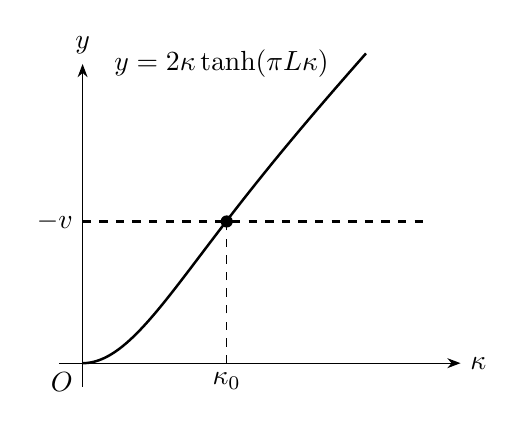
\begin{tikzpicture}[
  >=Stealth,
  font=\normalsize,
  axis/.style={line width=0.4pt},
  curve/.style={line width=0.9pt}
]
  % Axes
  \draw[axis,->] (-0.3,0) -- (4.8,0) node[right] {$\kappa$};
  \draw[axis,->] (0,-0.3) -- (0,3.8) node[above] {$y$};
  \node[below left] at (0,0) {$O$};

  % Horizontal line y = -v = |v| = 1.8
  \draw[curve,dashed] (0,1.8) -- (4.4,1.8);
  \node[left] at (0,1.8) {$-v$};

  % Curve y = 2*kappa*tanh(pi*L*kappa), scaled: let pi*L = 0.8, plot 1.1*x*tanh(0.8*x)
  \draw[curve,domain=0:3.6,samples=120]
    plot (\x, {1.1*\x*tanh(0.8*\x)});
  \node[above left] at (3.25,3.5) {$y = 2\kappa\tanh(\pi L\kappa)$};

  % Intersection point: 1.1*x*tanh(0.8*x) = 1.8 -> x ~ 1.815 (1.1*1.815*tanh(1.452) = 1.996*0.896 = 1.79 -> x=1.83)
  \fill (1.83,1.8) circle (2.2pt);
  \draw[axis,dashed] (1.83,0) -- (1.83,1.8);
  \node[below] at (1.83,0) {$\kappa_0$};
\end{tikzpicture}
\end{document}
